%\RequirePackage[l2tabu, orthodox]{nag}
\documentclass[12pt]{beamer}
\graphicspath{{Imagenes/}{../Imagenes/}}
\usepackage[utf8]{inputenc}
\usepackage[spanish]{babel}
\usepackage[autostyle,spanish=mexican]{csquotes}
\usepackage{hyperref}
\hypersetup{
  colorlinks=true,
  linkcolor=blue,          % color of internal links (change box color with linkbordercolor)
  citecolor=green,        % color of links to bibliography
  filecolor=magenta,      % color of file links
  urlcolor=cyan,           % color of external links
  linkbordercolor={0 0 1}
}
\usepackage{amsmath}
\usepackage{amsthm}
\usepackage{amsfonts}
\usepackage{multicol}
\usepackage{graphicx}
\usepackage{tabulary}
\usepackage{booktabs}
\usepackage{epstopdf}
\usepackage{media9}
\usepackage[binary-units=true]{siunitx}
\usepackage{standalone}
\usepackage{longtable}
\usepackage{bigints}
\usepackage{caption}
%\usepackage{enumitem}
\usepackage{tikz}
\usetikzlibrary{mindmap}
\usepackage[siunitx]{circuitikz}
\usetikzlibrary{arrows, patterns, shapes, decorations.markings}
\usetikzlibrary{matrix,positioning}
\tikzstyle{every picture}+=[remember picture,baseline]
\usepackage{color}
\usepackage{alltt}
\usepackage{verbatim}

\usepackage{fancyvrb}
\usepackage[os=win]{menukeys}
\usepackage{pifont}
\usepackage[sfdefault]{roboto}  %% Option 'sfdefault' only if the base font of the document is to be sans serif
%\usepackage[T1]{fontenc}
\setcounter{secnumdepth}{3}
\setcounter{tocdepth}{3}
\DeclareGraphicsExtensions{.pdf,.png,.jpg}
\renewcommand {\arraystretch}{1.5}
\definecolor{ao}{rgb}{0.0, 0.5, 0.0}
\definecolor{bisque}{rgb}{1.0, 0.89, 0.77}
\definecolor{amber}{rgb}{1.0, 0.75, 0.0}
\definecolor{armygreen}{rgb}{0.29, 0.33, 0.13}
\definecolor{alizarin}{rgb}{0.82, 0.1, 0.26}
\definecolor{cadetblue}{rgb}{0.37, 0.62, 0.63}
\newcommand*{\TitleParbox}[1]{\parbox[c]{6cm}{\raggedright #1}}%
\newcommand{\python}{\texttt{python}}
\newcommand{\textoazul}[1]{\textcolor{blue}{#1}}
\newcommand{\azulfuerte}[1]{\textcolor{blue}{\textbf{#1}}}
\newcommand{\funcionazul}[1]{\textcolor{blue}{\textbf{\texttt{#1}}}}
%\normalfont
\usepackage{ccfonts}% http://ctan.org/pkg/{ccfonts}
\usepackage[T1]{fontenc}% http://ctan.or/pkg/fontenc
\renewcommand{\rmdefault}{cmr}% cmr = Computer Modern Roman
\usefonttheme[onlymath]{serif}
\linespread{1.3}
\newcounter{saveenumi}
\newcommand{\seti}{\setcounter{saveenumi}{\value{enumi}}}
\newcommand{\conti}{\setcounter{enumi}{\value{saveenumi}}}

%reduce el tamaño de letra de la etiqueta equations
\makeatletter
\def\maketag@@@#1{\hbox{\m@th\normalfont\small#1}}
\makeatother

%se usa para la x en itemize
\newcommand{\xmark}{\text{\ding{55}}}

%\AtBeginDocument{\setlength{\tymin}{1em}}


\definecolor{myblue}{rgb}{.8, .8, 1}

\usepackage{amsmath}
\usepackage{empheq}

\newlength\mytemplen
\newsavebox\mytempbox

\makeatletter
\newcommand\mybluebox{%
    \@ifnextchar[%]
       {\@mybluebox}%
       {\@mybluebox[0pt]}}

\def\@mybluebox[#1]{%
    \@ifnextchar[%]
       {\@@mybluebox[#1]}%
       {\@@mybluebox[#1][0pt]}}

\def\@@mybluebox[#1][#2]#3{
    \sbox\mytempbox{#3}%
    \mytemplen\ht\mytempbox
    \advance\mytemplen #1\relax
    \ht\mytempbox\mytemplen
    \mytemplen\dp\mytempbox
    \advance\mytemplen #2\relax
    \dp\mytempbox\mytemplen
    \colorbox{myblue}{\hspace{1em}\usebox{\mytempbox}\hspace{1em}}}

\makeatother

\sisetup{separate-uncertainty}%


%Se usa la plantilla Warsaw modificada con spruce
\mode<presentation>
{
  \usetheme{Warsaw}
  \setbeamertemplate{headline}{}
  \useoutertheme{default}
  %\usecolortheme{beaver}
  \setbeamercovered{invisible}
}
%\AtBeginSection[]
%{
%\begin{frame}<beamer>{Contenido}
%\normalfont\mdseries
%\tableofcontents[currentsection]
%\end{frame}
%}

\setbeamertemplate{section in toc}[sections numbered]
\setbeamertemplate{subsection in toc}[subsections numbered]
\setbeamertemplate{subsection in toc}{\leavevmode\leftskip=3.2em\rlap{\hskip-2em\inserttocsectionnumber.\inserttocsubsectionnumber}\inserttocsubsection\par}
\setbeamercolor{section in toc}{fg=blue}
\setbeamercolor{subsection in toc}{fg=blue}
\setbeamertemplate{navigation symbols}{}
\setbeamercolor{frametitle}{fg=yellow,bg=blue!70!white}
\setbeamercolor{section in head/foot}{bg=gray!30,fg=red}
%\setbeamercolor{section in head}{bg=green,fg=red}
\setbeamercolor{subsection in head/foot}{bg=gray!30,fg=black}
\setbeamercolor{author in head/foot}{bg=gray!30}
\setbeamercolor{date in head/foot}{fg=blue}

%\mode<presentation>
%{
%  \usetheme{Warsaw}
%  \setbeamertemplate{headline}{}
%  %\useoutertheme{infolines}
%  \useoutertheme{default}
%  \setbeamercovered{invisible}
%  % or whatever (possibly just delete it)
%}

%\input{../Preambulos/pre_codigo}
\makeatletter
\setbeamertemplate{footline}
{
  \leavevmode%
  \hbox{%
  \begin{beamercolorbox}[wd=.333333\paperwidth,ht=2.25ex,dp=1ex,center]{author in head/foot}%
    \usebeamerfont{author in head/foot} \insertsection
  \end{beamercolorbox}}%
  \begin{beamercolorbox}[wd=.333333\paperwidth,ht=2.25ex,dp=1ex,center]{title in head/foot}%
    \usebeamerfont{title in head/foot} \insertsubsection
  \end{beamercolorbox}%
  \begin{beamercolorbox}[wd=.333333\paperwidth,ht=2.25ex,dp=1ex,right]{date in head/foot}%
    \usebeamerfont{date in head/foot} \textcolor{white}{\insertshortdate{}} \hspace*{2em}
    \textcolor{white}{\insertframenumber{} / \inserttotalframenumber}\hspace*{2ex} 
  \end{beamercolorbox}}%
  \vskip0pt%
\makeatother
\title{\large{Movimiento en un dimensión}}
\subtitle{Curso de Física}
\author[]{M. en C. Gustavo Contreras Mayén}
\date{\today}
\institute{Facultad de Ciencias - UNAM}
\titlegraphic{
\includegraphics[width=2cm]{../Imagenes/escudo-facultad-ciencias}\hspace*{4.75cm}~%
   
\includegraphics[width=2cm]{../Imagenes/escudo-unam}
}
\begin{document}
\maketitle
\section*{Contenido}
\frame[allowframebreaks]{\tableofcontents[currentsection, hideallsubsections]}
\fontsize{14}{14}\selectfont
\spanishdecimal{.}
\section{Movimiento en el plano}
\frame{\tableofcontents[currentsection, hideothersubsections]}
\subsection{Mecánica}
\begin{frame}
\frametitle{¿Qué es la mecánica?}
\begin{figure}
    \centering
    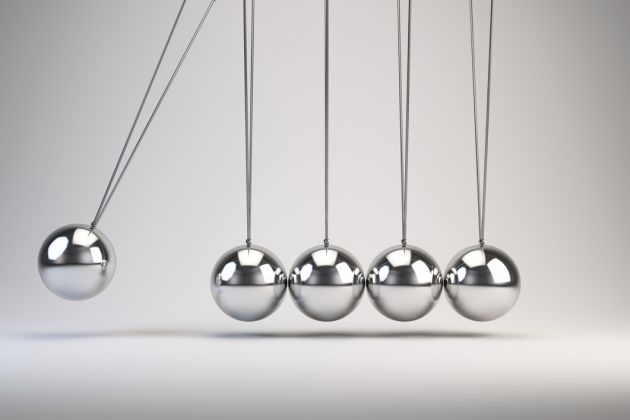
\includegraphics[scale=0.3]{./Imagenes/pendulo_newton.jpg}
\end{figure}
La mecánica estudia de las relaciones entre la fuerza, la materia y el movimiento.
\end{frame}
\begin{frame}
\frametitle{Áreas de la mecánica}
\begin{itemize}[<+->]
\item \textbf{Estática}: estudia el equilibrio entre las fuerzas.
\item \textbf{Cinématica}: es la parte de la mecánica que describe el movimiento sin atender las causas que lo originan.
\item \textbf{Dinámica:} estudia la relación entre el movimiento y sus causas, es decir, las fuerzas.
\end{itemize}
\end{frame}
\subsection*{Desplazamiento}
\begin{frame}
\frametitle{Estableciendo las referencias}
Tomemos como ejemplo un auto de carreras F1:
\begin{figure}
    \centering
    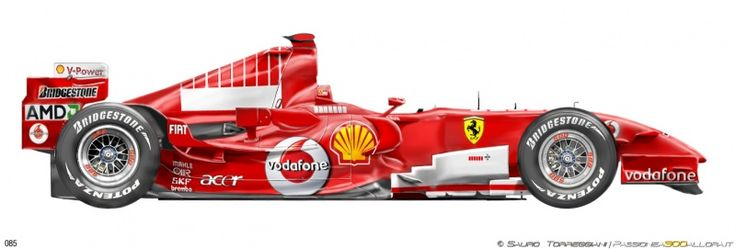
\includegraphics[scale=0.3]{./Imagenes/ferrari.jpg}
\end{figure}
\end{frame}
\begin{frame}
\frametitle{Eje coordenado}
Para estudiar su movimiento, necesitamos un sistema de coordenadas.
\\
\bigskip
\pause
Elegimos que el eje $x$ vaya a lo largo de la trayectoria recta del auto, con el origen $\mathbf{O}$ en la línea de salida.
\\
\bigskip
\pause
Representamos al auto como un punto, para considerarlo como un \textcolor{blue}{partícula}.
\end{frame}
\begin{frame}
\frametitle{Sistema de referencia}
\begin{figure}
    \centering
    \includestandalone{./Figuras/Ferrari_01}
\end{figure}
En este sistema de refencia podemos estudiar el movimiento de la partícula (el auto) sobre el eje $x$.
\\
\bigskip
Podremos estudiar el cambio de la posición (coordenadas en $x$) con respecto a un intervalo de tiempo.
\end{frame}
\begin{frame}
\frametitle{Cambios en la posición}
Supongamos que $\SI{1.0}{\second}$ después del arranque la partícula está en el punto $P_{1}$, a $\SI{19}{\meter}$ del origen, y que $\SI{4.0}{\second}$ después del arranque está en el punto
$P_{2}$, a $\SI{277}{\meter}$ del origen.
\\
\bigskip
\pause
El \textcolor{blue}{desplazamiento} de la partícula es un vector que apunta de
$P_{1}$ a $P_{2}$.
\end{frame}
\begin{frame}
\frametitle{Desplazamiento}
\begin{figure}
    \centering
    \includestandalone{./Figuras/Ferrari_02}
    \caption{Representación del cambio de posición de la partícula sobre el eje $x$.}
\end{figure}
\end{frame}
\begin{frame}
\frametitle{Definición de desplazamiento}
La componente $x$ del desplazamiento es simplemente el cambio en el valor de $x$:
\[ \mbox{desplazamiento } = P_{2}  - P_{1} = (277 - 19) = \SI{258}{\meter} \]
que hubo en el intervalo
\[ t_{2} - t_{1}  = 4.0 - 1.0 = \SI{3.0}{\second} \]
\end{frame}
\section{Velocidad media}
\frame{\tableofcontents[currentsection, hideothersubsections]}
\subsection{Definición}
\begin{frame}
\frametitle{Velocidad media}
Definimos la \textcolor{blue}{velocidad media} de la partícula  durante este intervalo de tiempo como una cantidad vectorial, cuya componente $x$, es el cambio en $x$ dividido entre el intervalo de tiempo:
\[ \mbox{velocidad media } = \dfrac{\SI{258}{\meter}}{\SI{3.0}{\second}} = \SI[per-mode=fraction]{86}{\meter\per\second}  \] 
\end{frame}
\begin{frame}
\frametitle{Velocidad media}
En el tiempo $t_{1}$ la partícula está en el punto $P_{1}$, con  coordenada $x_{1}$, para el tiempo $t_{2}$ está en el punto $P_{2}$ con la coordenada $x_{2}$.
\\
\bigskip
\pause
El desplazamiento de la partícula en el intervalo de $t_{1}$ a $t_{2}$ es el vector de $P_{1}$ a $P_{2}$.
\end{frame}
\begin{frame}
\frametitle{Velocidad media}
La componente $x$ del desplazamiento, denotada con $\Delta \: x$, es el cambio en la coordenada $x$:
\[  \Delta \: x = x_{2} - x_{1} \]
\pause
El intervalo de tiempo lo representamos como
\[ \Delta \: t = t_{2} - t_{1} \]
\end{frame}
\begin{frame}
\frametitle{Velocidad media}
La expresión para la velocidad media es entonces
\[ v_{\mbox{\tiny{media}}} = \dfrac{x_{2} - x_{1}}{t_{2} - t_{1}} = \dfrac{\Delta \: x}{\Delta \: t}  \]
\end{frame}
\subsection*{Gráfica de la velocidad media}
\begin{frame}
\frametitle{Gráfica de la velocidad media}
Podemos representar la posición del auto en función del tiempo, a través de una gráfica \textcolor{blue}{\emph{posición vs tiempo}}.
\\
\bigskip
\pause
\textbf{Nota: } La curva de la figura NO representa la trayectoria del auto. Ya que siempre es una línea recta.
\end{frame}
\begin{frame}[plain]
\frametitle{Gráfica de la velocidad media}
\begin{figure}
    \centering
    \includestandalone[scale=0.95]{./Figuras/Trayectoria_Ferrari}
\end{figure}
\end{frame}
\subsection{Interpretación gráfica}
\begin{frame}
\frametitle{Interpretación de la gráfica}
\begin{itemize}[<+->]
\item Los puntos $p_{1}$ y $p_{2}$ en la gráfica corresponden a los puntos $P_{1}$ y $P_{2}$ de la trayectoria del auto.
\item La línea $p_{1}$ - $p_{2}$ es la hipotenusa de un triángulo rectángulo con cateto vertical $\Delta \: x = x_{2} - x_{1}$ y cateto horizontal $\Delta \: t = t_{2} - t_{1}$.
\item La velocidad media del auto $v_{m} = \Delta \: x / \Delta \: t$ es igual a la pendiente de la línea $p_{1}$ - $p_{2}$ , es decir, el cociente del cateto vertical $\Delta \: x$ y el cateto horizontal $\Delta \: t$.
\end{itemize}
\end{frame}
\subsection*{Consideraciones}
\begin{frame}
\frametitle{Consideraciones}
La velocidad media depende sólo del desplazamiento total $\Delta \: x = x_{2} - x_{1}$ que se da durante el intervalo $\Delta \: t = t_{2} - t_{1}$ , no en los pormenores de lo que sucede dentro de ese intervalo.
\end{frame}
\begin{frame}
\frametitle{Consideraciones}
En el tiempo $t_{1}$ una motocicleta podría haber rebasado al auto en el punto $P_{1}$, para después reventar el motor y bajar la velocidad, pasando por $P_{2}$ en el mismo instante $t{2}$ que el auto.
\\
\bigskip
\pause
Ambos vehículos tienen el mismo desplazamiento en el mismo lapso, así que tienen la misma velocidad media.
\end{frame}
\section{Velocidad instantánea}
\frame{\tableofcontents[currentsection, hideothersubsections]}
\subsection{Definición}
\begin{frame}
\frametitle{Velocidad instantánea}
La velocidad media de una partícula durante un intervalo de tiempo no nos indica con qué rapidez, o en qué dirección, la partícula se estaba moviendo en un instante dado del intervalo.
\end{frame}
\begin{frame}
\frametitle{Velocidad instantánea}
Para describir el movimiento con mayor detalle, necesitamos definir la velocidad en cualquier instante específico o punto específico de la trayectoria.
\\
\bigskip
\pause
Ésta es la \emph{velocidad instantánea}, y debe definirse con cuidado.
\end{frame}
\subsection*{Expresión para la velocidad}
\begin{frame}
\frametitle{Expresión para la velocidad}
Para obtener la velocidad instantánea del auto (del ejemplo anterior) en el punto $P_{1}$, movemos el segundo punto $P_{2}$ cada vez más cerca del primer punto $P_{1}$ y calculamos la
velocidad media $v_{m} = \Delta \: x / \Delta \: t$ para estos desplazamientos y lapsos cada vez más cortos.
\end{frame}
\begin{frame}[plain]
\frametitle{Gráfica de la velocidad instantánea}
\begin{figure}
    \centering
    \only<1>{\includestandalone[scale=0.95]{./Figuras/Trayectoria_Ferrari_02}}
    \only<2>{\includestandalone[scale=0.95]{./Figuras/Trayectoria_Ferrari_03}}
    \only<3>{\includestandalone[scale=0.95]{./Figuras/Trayectoria_Ferrari_04}}
    \end{figure}
\end{frame}
\begin{frame}
\frametitle{Expresión para la velocidad}
Tanto $\Delta \: x$ y $\Delta \: t$ se hacen muy pequeños,  pero su cociente no necesariamente lo hace.
\\
\bigskip
\pause
En el lenguaje del cálculo, el límite de $\Delta \: x / \Delta \: t$ cuando $\Delta \: t$ se acerca a cero es la derivada de $x$ con respecto a $t$ y se escribe $\Delta \: x/ \Delta \: t$.
\end{frame}
\begin{frame}
\frametitle{Expresión para la velocidad}
La velocidad instantánea es el límite de la velocidad media conforme el intervalo de tiempo se acerca a cero.
\\
\bigskip
\pause
Es igual a la tasa instantánea de cambio de la posición con el tiempo. Usamos el símbolo $v_{x}$ , sin
\[ v_{x} = \lim_{\Delta \: t \to 0} \dfrac{\Delta \: x}{\Delta \: t} = \dfrac{dx}{dt} \]
\end{frame}
\begin{frame}
\frametitle{Dirección positiva o negativa de la velocidad}
Siempre suponemos que $\Delta \: t$ es positivo, así que $v_{x}$ tiene el mismo signo algebraico que $\Delta \: x$.
\\
\bigskip
\pause
Un valor positivo de $v_{x}$ indica que $x$ aumenta y el movimiento es en la dirección $x$ positiva; un valor negativo de $v_{x}$ indica que $x$ disminuye y el movimiento
es en la dirección $x$ negativa.
\end{frame}
\subsection*{Rapidez}
\begin{frame}
\frametitle{Rapidez}
La \textbf{rapidez} denota distancia recorrida dividida entre tiempo, con un régimen medio o instantáneo.
\\
\bigskip
\pause
Se escribe con el símbolo $v$ (sin subíndice) para denotar la rapidez instantánea, que mide qué tan rápido se mueve una partícula.
\end{frame}
\begin{frame}
\frametitle{Rapidez}
Por ejemplo, una partícula con velocidad instantánea $v_{x} = \SI[per-mode=symbol]{25}{\meter\per\second}$ y
otra con $v_{x} = -\SI[per-mode=symbol]{25}{\meter\per\second}$ se mueven en direcciones opuestas con la misma rapidez instantánea de $\SI[per-mode=symbol]{25}{\meter\per\second}$
\\
\bigskip
\pause
La rapidez instantánea es la magnitud de la velocidad instantánea, así que no puede ser negativa.
\end{frame}
\section{Aceleración}
\frame{\tableofcontents[currentsection, hideothersubsections]}
\subsection{Definición}
\begin{frame}
\frametitle{Definición}
Así como la velocidad describe la tasa de cambio de posición con el tiempo, \emph{la aceleración describe la tasa de cambio de velocidad con el tiempo}.
\\
\bigskip
\pause
Al igual que la velocidad, \textcolor{blue}{la aceleración es una cantidad vectorial}.
\end{frame}
\subsection{Aceleración media}
\begin{frame}
\frametitle{Aceleración media}
La aceleración describe la tasa de cambio de velocidad con el tiempo.
\\
\bigskip
\pause
Al igual que la velocidad, la aceleración es una cantidad vectorial.
\end{frame}
\begin{frame}
\frametitle{Aceleración media}
En el movimiento rectilíneo, su única componente distinta de cero está sobre el eje en que ocurre el movimiento.
\\
\bigskip
\pause
En el movimiento rectilíneo la aceleración puede referirse tanto a aumentar la rapidez como a disminuirla.
\end{frame}
\begin{frame}
\frametitle{Definición}
Supongamos que en el tiempo $t_{1}$, la partícula está en el punto $P_{l}$ y tiene una componente $x$ de velocidad (instantánea) $v_{1x}$, y en un instante posterior $t_{2}$ está en $P_{2}$ y tiene una componente $x$ de velocidad $v_{2x}$
\\
\bigskip
\pause
Así, la componente $x$ de la velocidad cambia en $\Delta \: v_{x} = v_{2x} - v_{1x}$ en el intervalo $\Delta \: t = t_{2} - t_{1}$ .
\end{frame}
\begin{frame}
\frametitle{Definición}
Se define la \textbf{aceleración media} de la partícula al moverse de $P_{1}$ a $P_{2}$ como una cantidad vectorial cuya componente $x$ es $a_{m}$ igual a $\Delta \: v_{x}$, el cambio en la componente $x$ de la velocidad, dividido entre el intervalo de tiempo $\Delta \: t$:
\pause
\begin{empheq}[box={\mybluebox[5pt][5pt]}]{equation*}
	a_{m} = \dfrac{v_{2x} - v_{1x}}{t_{2} - t_{1}} = \dfrac{\Delta \: v_{x}}{\Delta \: t}
\end{empheq}
\end{frame}
\begin{frame}
\frametitle{Unidades de la aceleración media}
Si expresamos la velocidad en metros por segundo y el tiempo en segundos, las unidades de la aceleración media están dadas en metros por segundo por segundo, o bien (\si[per-mode=symbol]{\meter\second\per\second}).
\\
\bigskip
\pause
Se escribe como  \si[per-mode=symbol]{\meter\per\square\second} y se lee \enquote{metros por segundo al cuadrado}.
\end{frame}
\subsection{Aceleración instantántea}
\begin{frame}
\frametitle{Aceleración instantánea}
Se puede definir la aceleración instantánea de la misma forma que se hizo con la velocidad instantánea.
\end{frame}
\begin{frame}
\frametitle{Aceleración instantánea}
Como ejemplo, supongamos que el carro de carreras  (una partícula) está en una recta como se muestra en la figura:
\begin{figure}
    \centering
    \includestandalone{./Figuras/aceleracion_01}
\end{figure}
\end{frame}
\begin{frame}
\frametitle{Definición de aceleración instantánea}
Para definir la aceleración instantánea en $P_{1}$, tomamos el segundo punto $P_{2}$ en la figura cada vez más cerca de $P_{1}$, de modo que la aceleración media se calcule en intervalos cada vez más cortos.
\end{frame}
\begin{frame}
\frametitle{Definición de aceleración instantánea}
La aceleración instantánea es el límite de la aceleración media conforme el intervalo de tiempo tiende a cero.
\\
\bigskip
\pause
En el lenguaje del cálculo diferencial, la aceleración instantánea es la tasa instantánea de cambio de la velocidad con el tiempo.
\end{frame}
\begin{frame}
\frametitle{Expresión para la aceleración instantánea}
\begin{empheq}[box={\mybluebox[5pt][5pt]}]{equation*}
	a_{x} =  \lim_{\Delta t \to 0} \dfrac{\Delta \: v_{x}}{\Delta \: t} = \dfrac{\Delta \: v_{x}}{\Delta \: t}
\end{empheq}
\pause
Vemos que se define la componente $x$ del
vector de aceleración o la aceleración instantánea.
\\
\bigskip
\pause
En el movimiento rectilíneo, las demás componentes de este vector son cero.
\end{frame}
\begin{frame}
\frametitle{La aceleración instantánea}
A partir de este momento, al hablar de \textcolor{blue}{aceleración} haremos referencia a la aceleración instantánea, no a la aceleración media.
\end{frame}
\end{document}